\documentclass[a4paper,openright,twoside,11pt]{report}

% % Include packages % %

% Basic
\usepackage[english]{babel}		% Document language
\usepackage[utf8x]{inputenc}	% Character encoding
\usepackage{appendix}			% Increases control of appendices

% Standard colors
\PassOptionsToPackage{dvipsnames}{xcolor}
	\RequirePackage{xcolor} % [dvipsnames]

% Figures
\usepackage{float}				% Improves handling of floating objects
\usepackage[pdftex]{graphicx}	% Improves handling of graphics
\usepackage{pdfpages}			% Allows inclusion of entire PDF
\usepackage{tikz}				% Allows construction of diagrams

% Tables
\usepackage{multicol}			% Allows multi-columns in tables
\usepackage{multirow}			% Allows multi-rows in tables

% Math
\usepackage{amsmath}			% Adds functionality to math environments
\usepackage{amssymb} 			% Adds to more symbols to math environments

% Listings
\usepackage{listings}			% Allows the use of listings

% Misc
\usepackage{xspace}				% Allows spaces after commands
\usepackage{todonotes}			% Enable todo notes
\usepackage{booktabs}			% Various optimizations to LaTeX
\usepackage{lastpage}			% Allows reference to LastPage 
\usepackage{type1cm}			% Increase flexibility of font sizes
\usepackage{enumerate}			% Allows one to choose the style of an enumeration
\usepackage[square,numbers]{natbib}
\bibliographystyle{unsrt}

% Hyperlinks
\usepackage[hyphens]{url}		% Create URL's with line breaks
\usepackage{hyperref}			% Allows hyperlinks
\usepackage{bookmark}

% Clever refs - although not clever enough to be included before hyperref....
\usepackage{cleveref}     % Adds intelligent references ("Figure F1-2", instead of "F1-2")

% ADD THESE LAST BECAUSE OF PACKAGE DEPENDENCIES!
%[LABEL] pagelayout
%[DESCRIPTION] Defines the page headers and whitespace placement.

%[BEGIN] Define page headers and footers
  %[BEGIN] Load fancy headers package
    \usepackage{fancyhdr}
  %[END]
  
  % Document visual header definition
	\setlength{\headheight}{15pt}
 	
 	\pagestyle{fancy}
	\renewcommand{\chaptermark}[1]{\markboth{\small{\scshape{#1}}\ \scshape{\small{\thechapter}}}{}}
	\renewcommand{\sectionmark}[1]{\markright{\scshape{\small{\thesection}}\ \small{\scshape{#1}}}}

	\fancyhf{}
	\fancyhead[LE,RO]{\thepage}
	\fancyhead[LO]{\rightmark}
	\fancyhead[RE]{\leftmark}
	
	\renewcommand{\headrule}{{\color{black}%
  \hrule width\headwidth height\headrulewidth \vskip-\headrulewidth}}
	\renewcommand{\headrulewidth}{0.3pt}
	\renewcommand{\footrulewidth}{0pt}

	\addtolength{\headheight}{0.5pt}
	\setlength{\footskip}{0in}
	\renewcommand{\footruleskip}{0pt}
	\fancypagestyle{plain}{%
		\fancyhead{}
		\renewcommand{\headrulewidth}{0pt}
	}
%[END]

%[BEGIN] Chapter customisation
  \usepackage{graphics}
  \usepackage{titlesec}
  \titleformat{\chapter}[display]
    {\normalfont\Large\raggedleft}
    {\MakeUppercase{\chaptertitlename}%
      \rlap{\resizebox{!}{1.5cm}{~\thechapter~} \rule{5cm}{1.5cm}}}
    {10pt}{\Huge\bf}
  \titlespacing*{\chapter}{0pt}{30pt}{20pt}
%[END]

%[BEGIN] Bibliography in TOC
  \usepackage[nottoc]{tocbibind} % Works only with standard classes
%[END]

%[BEGIN] Margin adjustment
  \usepackage[total={5in,8.75in},top=1in,left=1.5in,bottom=1.0in]{geometry}
%[END]

%[BEGIN] define whitespace placement
  \raggedbottom
%[END]

% Numbering
\renewcommand{\thesection}{\arabic{chapter}.\arabic{section}}
\renewcommand{\thesubsection}{\thesection.\arabic{subsection}}
\renewcommand{\thesubsubsection}{\thesubsection.\arabic{subsubsection}}
\renewcommand{\thefigure}{F\arabic{chapter}-\arabic{figure}}
\renewcommand{\thetable}{T\arabic{chapter}-\arabic{table}}

% Counters
\setcounter{tocdepth}{1}
\setcounter{secnumdepth}{3}
		% Layout definitions
% Part descriptions
% Usage \newpart{part name}{part text}
\newcommand{\newpart}[2]{
	\part[#1]{#1\\
		\begin{minipage}[c]{10cm}
		\centering
		\vspace{2cm}
		\normalsize{\textnormal{
			\textit{#2}
		}}
		\end{minipage}
	}
}

% Insert figure
\newcommand{\insertfigure}[4]{%
    \begin{figure}[H] %
        \center %
        \includegraphics[#1]{figures/#2} %
        \caption{#3} %
        \label{#4} %
        \vspace{-5pt}
    \end{figure} %
}

% Insert figure
\newcommand{\inserttexfigure}[3]{%
    \begin{figure}[H] %
        \center %
        \input{figures/#1} %
        \caption{#2} %
        \label{#3} %
        \vspace{-5pt}
    \end{figure} %
}

% Allow line break in texttt
\newcommand*\justify{%
  \fontdimen2\font=0.4em% interword space
  \fontdimen3\font=0.2em% interword stretch
  \fontdimen4\font=0.1em% interword shrink
  \fontdimen7\font=0.1em% extra space
  \hyphenchar\font=`\-% allowing hyphenation
}

\let\oldtexttt\texttt
\renewcommand*{\texttt}[1]{\oldtexttt{\justify #1}}

% Add Blankpage command
\newcommand{\Blankpage}{ %
    \newpage               %
    \thispagestyle{empty}  %
    \mbox{}                %
    \newpage               %
}

% TODO NOTES COMMANDS
\newcommand{\namedtodo}[5]
{
  \stepcounter{todocounter}
  \ifthenelse{\equal{#1}{inline}}
  % INLINE TODO
  {
    \todo[color=#4,caption={\textbf{\inserttodocounter #3: } #2},inline]
    {\textbf{\inserttodocounter #3: }\color{#5}#2}
  }
  % NORMAL TODO
  {
    \todo[color=#4,caption={\textbf{\inserttodocounter #3: } #2}]
    {\textbf{\inserttodocounter #3: }\color{#5}#2}
  }
}
% Counter format
\newcommand{\inserttodocounter}{\#\thetodocounter\;}

% FORMAT FOR TODO:
% [inline] (optional) besked navn bg-farve font-farve
\newcommand{\vagner}[2][]{\namedtodo{#1}{#2}{Vagner}{CarnationPink}{black}}
\newcommand{\thilemann}[2][]{\namedtodo{#1}{#2}{Stefan T}{NavyBlue!35}{black}}
\newcommand{\jesper}[2][]{\namedtodo{#1}{#2}{Jesper}{green}{black}}
\newcommand{\frederik}[2][]{\namedtodo{#1}{#2}{Frederik}{red!90}{black}}

%GIRAF commands
\newcommand{\giraf}{GIRAF\xspace}
\newcommand{\launcher}{Launcher\xspace}		% Custom commands and environments
% FIGURES
\graphicspath{{figures/}{../figures/}}

% Define hyperef style
\hypersetup %
{
	colorlinks=true,
	linktocpage=true, 
	pdfstartpage=1,
	pdfstartview=FitV,
	hypertexnames=true,
	pdfhighlight=/O,
	breaklinks=true,
	pdfpagemode=UseNone,
	pageanchor=true,
	pdfpagemode=UseOutlines,
	plainpages=false,
	bookmarksnumbered,
	bookmarksopen=true,
	bookmarksopenlevel=1,
	bookmarksdepth=2,
	urlcolor=NavyBlue,
	linkcolor=Red,
	citecolor=Red,
	pdfborder={0 0 0},
}

\lstset %
{
	language=Java,
	keywordstyle=\color{RoyalBlue},
    commentstyle=\color{Green}\ttfamily,
    stringstyle=\color{Red}\ttfamily,
	frame=shadowbox,
	framesep=5pt,
	aboveskip=1.5em,
	belowskip=1em,
	rulecolor=\color{blue!40!black},
	rulesepcolor=\color{white!93!black},
	basicstyle=\ttfamily\normalsize,
	numbers=left,
	numberstyle=\tiny,
	numberfirstline=true,
	numberblanklines=false,
%	showstringspaces=false,
	stepnumber=1,
	numbersep=9pt,	
	captionpos=b,
	escapeinside={(*}{*)},
	breaklines=true,
	breakatwhitespace=true,
	alsoletter={;}
}

% TIKZ
\usetikzlibrary{positioning,fit,calc,shapes,arrows,external,petri}
\tikzset{
    state/.style={
		rectangle,
		rounded corners,
		draw=black, very thick,
		minimum height=2em,
		inner sep=2pt,
		text centered
	},
    layer/.style={
		rectangle,
		rounded corners,
		draw=black, very thick,
		minimum height=4em,
    	minimum width=10cm,
		inner sep=2pt,
		text centered
   },
    dummy/.style={
		rectangle,
		rounded corners,
		minimum height=2em,
		inner sep=2pt,
		text centered
   },
	lbl/.style={
		above,
		sloped % make the text follow the path
	}

}

% Make quotes italic
\AtBeginEnvironment{quote}{\itshape}			% Package setup

% Only compile part of the report
% Useful if we want feedback on certain parts/chapters
%\includeonly{documents/01-Front/index,documents/03-Sprint1/index}

\begin{document}

% Remember to disable todonotes entirely in final version
% It can be done explicitly in preamble by passing 
% options [disable] to the todonotes package
\listoftodos

% Introduction
\pagenumbering{roman}
\pagestyle{empty}
%% Use this for frontpage image
%\includepdf[noautoscale]{figures/frontpage.pdf}
\phantomsection
\thispagestyle{empty}

\newcommand{\HRule}{\rule{\linewidth}{0.5mm}} % Defines a new command for the horizontal lines, change thickness here

\begin{center}
\textsc{}\\[0.5cm]

\textsc{\LARGE Aalborg Universitet}\\[0.8cm]
\textsc{\Large SW6 Project}\\[0.4cm]
\textsc{\large Developing Complex Software Systems}\\[0.4cm]

\HRule \\[0.4cm]
{ \huge \bfseries Software for Children with Autism}\\[0cm]
\HRule \\[0.8cm]
\begin{minipage}{0.4\textwidth}
\begin{flushleft} \large
\emph{Group:}\\
Jesper Byrdal Kjær\\
Frederik Bruhn Mikkelsen\\
Stefan Mailund Thilemann\\
Anders Vagner
\end{flushleft}
\end{minipage} 
~
\begin{minipage}{0.4\textwidth}
\begin{flushright} \large
\emph{Supervisor:}\\
Hua Lu
\end{flushright}
\end{minipage}\\[1.5cm]

%\includegraphics[width=\textwidth]{figures/legoCar.jpg}\\[1cm]

%{\large 20-12-2013}\\[0cm]

\vfill

\includegraphics[height=3cm]{figures/aauLogoEnStudent.png}
\vfill

\end{center}


\Blankpage
\phantomsection
\thispagestyle{empty}
% Titlepage [START]
    \sectionmark{Titlepage}

    \begin{tabular}{r}
        \parbox{\textwidth}{\raisebox{-15mm}{
\includegraphics[height=3cm]{figures/aauLogoEnStudent.png}} %
         \hfill \parbox{4.9cm}{ %
            \begin{tabular}{l} 
                {\textsf{\small{\textbf{Department of Computer Science}}}}\\
                {\textsf{\small{\textbf{Software 5th semester}}}}\\
                {\textsf{\small{Address: Selma Lagerlöfs Vej 300}}} \\
                {\textsf{\small{\hspace{13 mm} 9220 Aalborg Øst }}} \\
                {\textsf{\small{Phone no.: 99 40 99 40}}} \\
                {\textsf{\small{Fax no.: 99 40 97 98}}} \\
                {\textsf{\small{Homepage: \url{http://www.cs.aau.dk}}}}
            \end{tabular}}}
    \end{tabular}
    
    \begin{tabular}{cc}
	
        \parbox[3cm]{7cm}{ %
	\vspace{7mm}
            \begin{description}
                \item {\textbf{Project title}:} \\
                    Software for Helping \\
                    Children with Autism
                    \hspace{4cm}
                \item {\textbf{Subject}:} \\
                  Developing Complex \\
                  Software Systems
            \end{description}
	\vspace{-4mm}
            \parbox{8cm}{ %
                \begin{description}
                    \item {\textbf{Project periode}:} \\
                        Spring 2014
                    \hspace{4cm}
                    \item {\textbf{Group name}:} \\
                        SW605F14
                    \hspace{4cm}
                    \item {\textbf{Supervisor}:} \\
                        Hua Lu
                    \item {\textbf{Group members}:}\\%\newcommand{\sh}{18pt}\\%
                    Jesper Byrdal Kjær\\[0.20cm]
                    Frederik Bruhn Mikkelsen\\[0.20cm]
					Stefan Mailund Thilemann\\[0.20cm]
					Anders Vagner
                \end{description}
            }
	    \vspace{-4mm}
            \begin{description}
                \item {\textbf{Copies}:} XX
                \item {\textbf{Pages}:} \pageref{LastPage}
                \item {\textbf{Appendices}: XX} 
                \item {\textbf{Finished}: XX} 
            \end{description}
            \vfill 
        } &
        \parbox{7cm}{ %
            %\vspace{.15cm} %
            \hfill %
            \begin{tabular}{l}%
                {\textbf{Abstract}:}\bigskip \\%
                \fbox{ %
                    \parbox{6.2cm}{\bigskip %
                    {\vfill{\small %
                     \thilemann[inline]{Insert text here...}
                        \bigskip}}%
                    }}%
            \end{tabular}%
        }
    \end{tabular}

    \noindent{\footnotesize\emph{The material in this report is freely and publicly available, publication with source reference is only allowed with authors' permission.}}
% Titlepage [END]
\Blankpage

\newcommand{\headerPreface}{Preface}
\cleardoublepage
\phantomsection
\pdfbookmark{\headerPreface}{chap:preface}
\chapter*{\headerPreface}\label{chap:preface}
This report is created by Software Engineering students as a Bachelor project at Aalborg University, spring semester 2014.
To read and understand the report, it is expected that the reader has a background in Computer Science in the light of the technical contents.


Since multiple project groups are collaborating towards developing a complete system, the structure of this report is divided into chapters that logically follows from working in sprints specified by the multi-project guidelines.
Thus there is a chapter for each sprint, which is further subdivided into:

\thilemann{Maybe add small description of each section}

\begin{itemize}
\item Sprint Overview
\item Analysis and Design
\item Developments
\item Sprint Review
\end{itemize}

Following the chapters describing the four sprints, \cref{chap:collaboration} focuses on the work that is done in collaboration with other groups.
Lastly, the results of the project is presented in \cref{chap:evaluation}.

References and citations is given with number notation, for example \thilemann{Indsæt eksempel på cite her.}. 
When writing "we", it is referring to the members of the project group.

\thilemann[inline]{Please give thanks where thanks is due...}


% Some setup
%\setcounter{page}{4}
\setcounter{secnumdepth}{3}

\cleardoublepage
\phantomsection

%Table of content
\pdfbookmark{\contentsname}{toc}
\setcounter{tocdepth}{1}
\tableofcontents

\clearpage

% Input contents
\pagestyle{headings}
\pagenumbering{arabic}
% Use include to do some latex magic when working on big reports
% Switches to temp .aux file to avoid recompilation of entire project
\newcommand{\headerIntroduction}{Introduction}
\chapter*{\headerIntroduction}\label{chap:introduction}
\addcontentsline{toc}{chapter}{\headerIntroduction}

The desire for the latest technology, whether it be a new car that enhances the safety of driving it, a gesture enabled television set or the constant craving for the latest mobile phones and tablets, often reflects a wish of improving certain areas of our lives using technology.
This reports focuses on improving the way-of-life of children diagnosed with different kinds of \textit{Autism Spectrum Disorders} (ASD), including autism and Asperger syndrome.
This is achieved by developing an Android software suite for tablets called \giraf, consisting of tools that strives to replace some of the children's daily routines.
It could for example be an interactive application that guides the children in putting on their outdoor clothes in the best order, or a game that focuses on improving the speech of speech-impaired children (referring to XXX and Cars respectively, which is included in \giraf).

~\linebreak[2]

Comply with:
Study Regulations
Autism Spectrum Disorder ASD

An emphasis in the study 
regulation is on solving realistic problems

The development of the systems and the requirements for it must be based on the ideas and needs of 
the costumers. The focus of the semester is on producing a functional and running product.


......These disorders are characterized by social deficits and communication difficulties, stereotyped or repetitive behaviors and interests, and in some cases, cognitive delays.

%\newpart{Sprints}{This is a very small descriptive text that introduces the part... It is sooo nice!}
%\label{part:sprints}

\chapter{First Sprint}

\section{Sprint Overview}
\thilemann{Please rewrite text below to make fit new structure.}

\subsection{Planning}

\subsection{Objectives}
The first sprint lasted from the \vagner{date} till the \vagner{date}.
In the following we will describe the tasks we worked on during this phase of the project period. 
Central activities in the sprint were getting to know the existing codebase, setting up the tools to be used, and initiating the cooperation with the contact persons.

We worked on the system component known as \textit{\launcher}, an interface for accessing other \giraf applications on the device.
Resolving pre-exisiting issues in the program was the main focus - as these were being resolved, focus shifted towards refactoring source code, improving the user experience and the functionality of the application.
The sprint ended with a fully operational \launcher, versioned with the other components of the project.\jesper{What do we mean by this?}

\section{Analysis and Design}
\section{Launcher}
Launcher is an application in the GIRAF application suite.
The main purpose of Launcher is to provide a user-friendly means of accessing other applications in the GIRAF suite, as well as regulating access to these applications, based on a user system.

\subsection{Motivation for Working with Launcher}
Launcher was originally developed by Andersen et al. in 2011 \cite{launcher2011}, and refined further by Andersen et al. in 2012 \cite{launcher2012}.
On an opening meeting however, the costumer contact persons made us aware that they rarely used Launcher, as it had proven to be unreliable and often would crash. 
They preferred to access the GIRAF applications through the Android tablets own interface.
The control committee of the multi-project decided that the focus of the first sprint should be on debugging, and as Launcher was a relatively complete, but was reported as unreliable, an obvious focus for the sprint was debugging. 
A separate project group was tasked with handling all negotiations with the customers during this first sprint, in order to compile a backlog for the second sprint.
Therefore, we were to attempt to resolve all issues, that we could clearly identify as issues, without having to discuss them with the costumer.\vagner{We kinda did slightly more than this, ye?}

\subsection{Launcher Functionality}
The functionality of Launcher can be summed up through a description of its four activities:
\begin{itemize}
	\item The \textit{Logo activity} shows the GIRAF logo, while loading the subsequent activities.
	\item The \textit{Authentication activity} requires the user to authenticate him- or herself before proceeding. 
	Andersen et al. (2012) describes how user identification is necessary, as the GIRAF settings must be able to vary from user to user. 
	The report furthermore describes how autistic children might have problems with a traditional username-password system. 
	Therefore, the authentication activity is based on a QR-scanner, where each child and guardian has a small brick with a QR-code they scan to identify 		  	themselves. 
	The activity loads the user information from the database, and proceeds to the \textit{Home activity}.
	\item The \textit{Home activity} allows the user to launch the available GIRAF applications. 
	The availability of an applications depends on whether the application exists locally on that device, and on whether the user is marked in the database as 	having rights to that application. 
	Furthermore, a number of widgets allows the user to see the synchronization status of the local database in relation to the remote database, and the 	 	date. 
	There is also a button that allows to user to log out, and return the \textit{Authentication activity}. 
	Finally, there is a colour palette hidden in a drawer component, where the user can change the base colour of applications. 
	The idea is make it easier for the children to differentiate different applications. 
	Ideally the choice of colour should also reflect in the application launched from the icon, giving the child consistent visual associations throughout GIRAF.
	The latter is implemented in the \textit{Timer} application.\vagner{Add a source to this}
	\item The \textit{Profile Select activity} is started when a guardian launches an application from Launcher. 
	It displays a list of all children associated with this guardian, allowing him or her to choose which child's profile to use when launchiung the selected 	 		 	application. 
	When a child is selected, the application launches, omitting the \textit{Profile Select activity}.
\end{itemize}\vagner{When referring to the different activities in subsequent sections, we should refer to this section imo}



\section{Drawer}
The drawer is the part of the Launcher that allows users to give their installed apps a new color.
It is available in the \lstinline{HomeActivity} activity.

The drawer is a bar in the left side of the screen, several smaller widgets on it.
These widgets are the \lstinline{GWidgetCalendar}, the \lstinline{GWidgetConnectivity} and the \lstinline{GWidgetLogout} - they are widgets originating from the \lstinline{OasisLib} project group.

When the bar is manipulated with, it can be placed further towards to center of the screen, revealing a panel with colours.
Illustrations of the drawer in open and closed form can be seen on figure \vagner{insert} and figure \vagner{insert}, respectively.

While the drawer worked as intended, there were a number of improvements desired to be implemented.
This section describes the original drawer, the desired improvements and the improved drawer.

\subsection{The original drawer}

The original drawer would open by pressing and holding the bar and sliding it to the right.
While being opened, the drawer would push the apps along with it to the right, resulting in some apps going out of reach.
Furthermore, the drawer would stop when pressure was released from the touchscreen, meaning it could be left in a half-opening, half-closed state.
To change the colour of an app, a colour could be drag-and-dropped onto an app, changing its colour.

The code working this animation was based on an \lstinline{OnTouchListener}, focusing mainly on the \lstinline{MotionEvent.ACTION_MOVE} event.
\lstinline{MotionEvent.ACTION_MOVE} would set the position of the entire drawer, panel and bar, to the exact point it had currently been moved to and redraw the elements.
Because the \lstinline{ScrollView} containing the apps was set to \lstinline{android:layout_toRightOf} in the .xml files for the layout, the \lstinline{ScrollView} would adjust itself to the new position each time the event fired.

The panel of colours was implemented using a \lstinline{GridView} - using the command \lstinline{AppColors.setAdapter(new GColorAdapter(this));} would set the \lstinline{GColourAdapter} from the \lstinline{OasisLib} group would create the correct panel.

Selecting a colour and assigning it to an app worked by means of an \lstinline{OnDragListener} called \lstinline{GAppDragger}.

\subsection{Desired improvements}

Since the project group had yet to have a meeting with the customer, these improvements are based on the groups desires.
Originally, the following improvements were desired :

\begin{itemize}
\item The drawer should either be opened or closed - a half-open or half-closed state should result in the drawer popping into the closest option.
\item The drawer should close while a color was being dragged and opened again when the color was dropped.
\item The drawer should not push the apps outside of the screen.
\end{itemize}

When work started, however, additional improvements were found to be desireable:

\begin{itemize}
\item The animation of the drawer and the code positioning all of the elements in \lstinline{HomeActivity} should be refactored in order to:
\begin{itemize}
\item take advantage of standard Android animations and code standards.
\item allow the activity to dynamically adjust according to screensize.
\item reduces the amount of clutter in the code and improve readability of the code.
\end{itemize}
\item An icon indicating opening and closing functionality of the drawer should be placed on the bar.
\end{itemize}

All of these improvements were implemented before the end of the first sprint. \vagner{verify this is the case when the sprint is done.}

\subsection{The improved drawer}

Opening and closing the improved drawer was implemented with an \lstinline{OnTouchListener} through the \lstinline{MotionEvent.ACTION_DOWN} event and a standard Android \lstinline{TranslateAnimation}.
Pressing the bar fires the event and and begins the animation.
A \lstinline{boolean} variable determines whether the drawer was opened or closed when the event fired and thus if the animation should translate left or right.
By also adding an \lstinline{OnDragListener} to the drawer, the animation would also play when dragging and dropping colours from the panel; closing the drawer on \lstinline{DragEvent.ACTION_DRAG_STARTED} and opening it again on \lstinline{DragEvent.ACTION_DRAG_ENDED}.

Having the \lstinline{ScrollView} containing the apps stay during the animation is linked to the refactoring of the code positioning elements in the activity.
Previously, all elements were merely declared in the .xml file, while positioning of the elements was statically set in the \lstinline{HomeActivity} load code - over100 lines of parameter setting code.\vagner{maybe not include mocking the previous group?}
This was refactored to have the all positioning declared dynamically depending on screen size, apart from positioning of the \lstinline{ScrollView}.\vagner{Stefan, write intelligent stuff about dynamic positioning of the ScrollView}
\vagner{Add documentation about the icon indicating opening and closing of the drawer}

The improved drawer fullfills all desired improvements in Sprint 1 and provides a smoother and more pleasant experience for the user, while refactoring of the acting code provides clarity and readability of developers.
\section{Testing}\label{sec:testing_sprint1}

As one of our goals was to increase the reliability of Launcher, we decided to conduct functional testing on the application.
We studied the specifications formulated by the earlier development teams in their 2011 \cite{launcher2011} and 2012 \cite{launcher2012} reports, and then studied how well Launcher corresponded to these specifications, by using the program in a number of different ways. 

Furthermore, a number of test cases were not based directly on the old specifications, but on what we found reasonable to expect of the application, based on our own knowledge of the system.

The tests described here were all performed by operating the running application, and were explicitly not based on our knowledge of the source code. 
This characterises our tests as dynamic black box testing. 

A number of test cases that would have been relevant, were not performed in this sprint, as they would have been too time consuming. 
These tests required significant changes to the test data built into the GIRAF system, or repeatedly installing and uninstalling applications from the device.
As there, at the time, was no central repository of stable application builds, most of the time would be spent building, installing and resetting different applications.

We only describe the results we found most interesting in this section, mainly tests that failed in a significant way. \jesper{Should we have a test appendix with the full results?}\vagner{I think so.}

\subsection{Specifications}
In the 2011 report by Andersen et al. \cite{launcher2011} the following specification for Launcher is presented:
\begin{quote}
\begin{itemize}
	\item \textit{List only applications that is part of the GIRAF system.}
	\item \textit{List on applications that the user is able to use, according to the user's capabilities.}
	\item \textit{List only applications if their usage is not limited by the current location or time.}
	\item \textit{Only display application names if the user is able to read.}
\end{itemize}
\end{quote}

Common to all these, is that they were either difficult to test, or simply not implemented (some may have been implemented to some degree in 2011, but then removed by the 2012 team). The difficulty stems from the necessity of manipulating test data, that is hard coded into the local database of each device. We decided it would be more reasonable to revisit these test cases when GIRAF's database system became ready for use.

The 2012 report by Andersen et al. \cite{launcher2012} contains no explicit specifications, but does contain a list of use cases. We used these as the basis of our tests:
\begin{quote}
\begin{itemize}
	\item \textit{New guardian log in.}
	\item \textit{Configuring an app for a child.}
	\item \textit{Launching an app for a child in guardian mode.}
	\item \textit{Letting a child use an app for a limited time.}
\end{itemize}
\end{quote}
Note that their report also contains an explanation of each use case. We leave these out for brevity.








\section{Developments}
\subsection{Test Results}
Below is shown a selection of our test cases and their results.
As mentioned in the introduction of this section, we will only discuss the most interesting results, i.e. tests that led to discovery of significant issues.

\subsubsection*{Changing the Colour of an Application Icon}
\paragraph{Specification:} Configuring an app for a child.
\paragraph{Test case:} Use the colour drawer to change the colour of an application, and check if the change is applied to both the application's icon, and its own user interface. (Some applications do not support changing the colour of their user interface.\jesper{Det her skal vi lige være sikre på.})
\paragraph{Result:} The colour of the icon changed immediately, but when starting the application, it still used the pre-change colour. A little experimenting showed that the change is not applied to the application until the user logs into Launcher again.
\paragraph{Resolution:} The issue was resolved, and the change in colour is now reflected in the application immediately.

\subsubsection*{Applications that Crash Launcher}
\paragraph{Specification:} Launching an app for a child in guardian mode.
\paragraph{Test case:} Open an application with a random child profile selected in the profile selector.
\paragraph{Result:} While not directly related to the intent of the use case, while running the test, we attempted to open what turned out to be a non-working version of a GIRAF application. The application suffered an unhandled exception, causing both it and Launcher to crash. This is not satisfactory, as Launcher should always work on top of the device operating system, denying the children access to device settings when using the device without supervision.
\paragraph{Resolution:} The issue was resolved, by making Launcher catch all exceptions thrown by the GIRAF applications it hosts.

\subsubsection*{Use of Device Buttons}
\paragraph{Specfication:} The device buttons (\textit{Back}, \textit{Home}, and \textit{Multitasking}) should have no effect in the \textit{Logo} and \textit{Authentication} activities, as the user should not be able to ``back out'' of Launcher to the device OS.
\paragraph{Test case:} Use the device buttons in different activities and situations.
\paragraph{Result:} In both the \textit{Logo} and \textit{Authentication} activities, applying the \textit{Home} and \textit{Back} buttons made Launcher restart. The \textit{Multitasking} button always activates the multitasking screen of the device OS.
\paragraph{Resolution:} The \textit{Back} button was suppressed. We were however unable to find a similar method for suppressing the other two buttons. This issue was postponed to a later sprint, when it would be easier to determine if it is worth spending the time needed to solve it.
\subsection{The Authentication Animation}
The first time we attempted to start Launcher, we found that it was unable to do so, as the application crashed, and logged an \lstinline{OutOfMemoryError}.
It turned out that the problem was caused by an animation in the \textit{Authentication} activity, implemented as an instance of the Android class \lstinline{AnimationDrawable}, a class designed to create animations from a sequence of images.
According to the documentation for Android \cite{androidreference}, the existing implementation was technically correct, but the error persisted.

After some investigation we found that when the instance of \lstinline{AnimationDrawable} is created, it loads the entire sequence of images into the main memory at once.
The images are compiled with the application in the compressed Portable Network Graphics (PNG) format.
However, as they are loaded, Android converts each image to a 32-bit bitmap, which is 4 bytes per pixel, making the images take up about 20 times more space, and the entire animation use about 40 MB of memory. We hypothesized that this was the source of the \lstinline{OutOfMemoryError}.

Our solution to this problem was to create a new class which simulates the behaviour of \lstinline{AnimationDrawable}, but uses the original PNG images.

The original \lstinline{AnimationDrawable} was set up as shown in \Cref{lst:animationDrawable}. \lstinline{R.animator.instruct_ani} is a list of images combined with a constant for each image, which determines the duration each image should be shown.

\begin{lstlisting}[caption={The original animation implementation, using \lstinline{AnimationDrawable}.},label={lst:animationDrawable}]
final ImageView instructImageView = (ImageView) findViewById(R.id.animation);
instructImageView.setBackgroundResource(R.animator.instruct_ani);

instructImageView.post(new Runnable(){
    @Override
    public void run(){
        AnimationDrawable anim = (AnimationDrawable) instructImageView.getBackground();
        anim.start();
    }
});
\end{lstlisting}

Our class, simulating \lstinline{AnimationDrawable}, has the method \lstinline{play()}, shown in \Cref{lst:methodPlay}, where the input parameter \lstinline{pFrameNo} is the initial image in a static array which contains all the images used in the animation. 
With this method we only keep one image in memory at all times, since we are changing the image for each run of the \lstinline{play} method and there by avoid an out of memory error.
\begin{lstlisting}[caption={Our method for playing an animation based on a set of images.},label={lst:methodPlay}]
private void play(final int pFrameNo){
    mImageView.postDelayed(new Runnable(){
        @Override
        public void run() {                    
            mImageView.setImageResource(mFrames[pFrameNo]);

            if(pFrameNo == mLastFrameNo)
                play(0);
            else
                play(pFrameNo + 1);
        }
    }, mDuration);
}        
\end{lstlisting}

After we switched the old \lstinline{AnimationDrawable} implementation with our new class, the problem disappeared.
\section{Launcher Debug Mode}
When opening Launcher you are immediately presented to the \lstinline|LogoActivity| activity, which shows a loading animation for a specified amount of time, based on \lstinline|public static final int LOGO_ANIMATION_DURATION = 2000;| from the \lstinline|Constants| class.
The nature of Launcher also requires the user to authenticate himself when starting the application to gain access to the suite of installed \giraf applications on the device.
These design decisions imposes us as developers to significant wait times; recompiling and thus restarting Launcher time and again, emphasizes on this fact.

\thilemann{We should add a sequence diagram - but maybe not here...}
\thilemann{Maybe also a class diagram to give an overview?}

To overcome the examples just described, it is decided to implement a debug mode to simplify and quicken the process of working with Launcher.
Debug mode is controlled from the \lstinline|LogoActivity| class by setting the local fields below:

\begin{itemize}
\item Enable or disable debug mode entirely, overriding other settings:\\
\lstinline|private final boolean DEBUG_MODE = true;|
\item Skip \lstinline|AuthenticationActivity| activity:\\
\lstinline|private final boolean showAuthentication = false;|
\item Skip the animation on \lstinline|LogoActivity| activity:\\
\lstinline|private final boolean showLogoAnimation = false;|
\item Login either as a guardian or child when skipping authentication:\\
\lstinline|private final boolean loginAsChild = false;|
\end{itemize}

When the above fields are set, debug mode is enabled globally in Launcher from the \lstinline|onCreate| method in \lstinline|LogoActivity| through the call showed in \cref{lst:debugmode:enable}.

\begin{lstlisting}[caption={Enable debug mode from \lstinline|LogoActivity|.},label={lst:debugmode:enable}]  
if(DEBUG_MODE)
  LauncherUtility.enableDebugging(DEBUG_MODE, loginAsChild, this);
\end{lstlisting}

The \lstinline|enableDebugging| method is seen in \cref{lst:debugmode:enablemethod}.
It needs a reference of the calling activity to show debug information on the active activity.

\begin{lstlisting}[caption={Enable debug mode by calling \lstinline|enableDebugging|.},label={lst:debugmode:enablemethod}]  
public static void enableDebugging(boolean debugging, boolean loginAsChild, Activity activity) {
  DEBUG_MODE = debugging;
  DEBUG_MODE_AS_CHILD = loginAsChild;

  ShowDebugInformation(activity);
}
\end{lstlisting}

The code in \cref{lst:debugmode:show}............


\begin{lstlisting}[caption={Show a debug information on activity if debug is enabled.},label={lst:debugmode:show}]  
public static void ShowDebugInformation(Activity a) {
  if (DEBUG_MODE) {
    LinearLayout debug = (LinearLayout) a.findViewById(R.id.debug_mode);
    TextView textView = (TextView) a.findViewById(R.id.debug_mode_text);
    textView.setText(a.getText(R.string.giraf_debug_mode) + " " + (DEBUG_MODE_AS_CHILD ? a.getText(R.string.giraf_debug_as_child) : a.getText(R.string.giraf_debug_as_guardian)));
    debug.setVisibility(View.VISIBLE);
    try {
      Thread.sleep(200);
    } catch (InterruptedException e) {
      e.printStackTrace();
    }
  }
}
\end{lstlisting}

\section{Minor Bugs}

There were several minor bugs, anomalies and things that did not work, when the sprint was started.
These being minor issues, do not warrant their own sections - however it is worth mentioning some of the problems solved.

\subsection*{Inconsistant UI in \lstinline{ScrollView} of \lstinline{ProfileSelector} activity}

The \lstinline{ScrollView} of the \lstinline{ProfileSelector} activity would overlap the rounded corners of the view when scrolling.
The issue was resolved by overlaying a shape with the corners rounded and a transparent center on the Listview.

\subsection*{Highlighting and Dehighlighting apps when dragging colour}

It was desired to have visual effect for when a colur was dragged over an app.
This achieved by scaling up the app being dragged over by 10\% on \lstinline{DragEvent.ACTION_DRAG_ENTERED} and scaling it down again on \lstinline{DragEvent.ACTION_DRAG_EXITED} and \lstinline{DragEvent.ACTION_DRAG_ENDED}.

\subsection*{Loading Animation on startup}

The previous group expressed that a loading animation when starting Launcher should be available.
This was made by defining a custom animation \lstinline{logoanimation.xml} and launching the animation on startup.

\subsection*{Back button functionality}

While the starting animation plays in \lstinline{LogoActivity} and while on the login screen in \lstinline{AuthenticationActivity}, it should not be possible to use the back button on the tablet.
The issue was resolved by overriding the back button to have no effect in those activities.

\subsection*{Child Mode}

Regardless of being logged in on a child or guardian profile, Launcher would open the \lstinline{ProfileSelector} before opening any app.
It should only open that activity, while in a guardian profile was logged in.
The issue was solved by checking the \lstinline{getRole()} parameter of a profile and then appropiately override the \lstinline{OnClickListener} depending on the role. 

\subsection*{Horizontalize the app}

The Launcher was the only app able to enter portrait mode - all other apps where configured to work in landscape mode.
The \lstinline{AndroidManifest.xml} for the launcher was edited to only allow landscape mode for all activities.

\subsection*{Bugs related to other groups}

There were two bugs found related to other groups than our own.
We did not fix these bugs, but simply reported them to the corresponding groups.

\begin{itemize}
\item The \lstinline{GButton} widget from the GUI group would crash any activity it was used in
\item Danish characters would not decode correctly from the database.
\end{itemize}

There were other, smaller issues, not described in this section.
They were however deemed insignificant.

\section{Sprint Review}
As we are using the Scrum method of development for the entire \giraf project, a sprint review meeting was planned for the end of the iteration. 
Larman \cite[p. 71]{larmanAgile} describes this type meeting as follows:
\begin{quote}
``At the end of each iteration, there is a review meeting (maximum of four hours)
hosted by the Scrum Master.
The team, Product Owner, and other stakeholders attend.
There is a demo of the product.

Feedback and brainstorming on future directions is encouraged, but no commitments are made during the meeting.
Later at the next Sprint Planning meeting, stakeholders and the team make commitments."
\end{quote}

At our meeting, the Scrum master of the \giraf project started with a short presentation, and then gave the floor to the groups\jesper{Describe the context of the GIRAF project early in the report.}, who spent five minutes each demonstrating their progress to the stakeholders\jesper{In aforementioned context description, define the stakeholders of the GIRAF project}. 
After the demonstrations, the stakeholders left, and groups proceeded to distribute the sub-projects among them, in preparation for the second sprint.

We do not consider this sprint review meeting a success, due to the following reasons:
\begin{itemize}
	\item It was a one-way meeting, where the stakeholders were presented with the progress, but were not encouraged to give any feedback. As a result, the development teams had no gain from the meeting, and were ill prepared for the second sprint. This problem was exacerbated by the lack of the sprint planning meetings required in Scrum to start a new sprint. As Larman \cite[p. 70]{larmanAgile} describes, during the sprint planning meetings goals are re-prioritized, and a new sprint backlog is created. 
	\item Several of the demonstrations had technical problems, such as applications crashing in the emulator used for the demonstration. This surprised the presenting groups, and thus they were unable to demonstrate their actual progress. A related problem was that several groups did not direct their presentation towards the costumers, and therefore focused on technical details, using a very technical vocabulary. The demonstration should be better prepared, with more focus on the actual goal of the meeting.
	\item Not all stakeholders were able to attend, as the meeting planned at a relative late date. As the main goal of the meeting is for the stakeholders review the progress of the project, this is not optimal.
\end{itemize}

These problems were discussed after the conclusion of the meeting. IT was suggested that a possible root problem was the \giraf Scrum master being overworked with planning this meeting along with his other responsibilities. It was decided to, at a later date, discuss the possibility of designate another person as responsible for conducting the sprint review meeting, and possibly the sprint planning meetings.

As a consequence of the lacking feedback, the \launcher sub-project had no clear goals for the second sprint, as most obvious issues had been resolved during the first sprint. We therefore decided get in contact with one of the costumers early in the second sprint, and discuss Launcher. We then expected to able to build a backlog for the second sprint along with this costumer. This is not an optimal solution, as the backlog should be compiled and prioritized as part of a coherent development process. But this solution will at least give us the ability to work from the requests of a costumer, rather than from what we ourselves think the costumers want. This costumer contact will be discussed further in \jesper{Ref til afsnit om kundekontakt, sprint 2.}



\chapter{Second Sprint}
As the described in \cref{sec:sprint1:review}, the end of the first sprint left us unsure of whether there was more work to be done on \launcher, and if so, what this work could be. 
We decide that it is necessary to arrange a meeting with some of the clients, in part to hear their thoughts on the current version of \launcher, and in part to discover new features.
During the first sprint we informally discussed ideas for new features.
These features include an improved format for the profile selector, and a new Settings application, providing a uniform interface for changing settings across all applications. 
To provide a good foundation for presenting and discussing these ideas with the customers, we design a number of prototype drawings of how our ideas could be realized.

A separate important issue in this sprint is adapting \launcher for new versions its dependencies. 
The \textit{OasisLib} library underwent drastic changes at the end of the first sprint, which unfortunately resulted in several applications, including \launcher, being unable to run.

In summary, the main points of this sprint are:

\begin{itemize}
\item Description of the designed prototypes in \cref{sec:sprint2:analysis}, with summaries of the first meeting in \cref{sec:sprint2:firstmeeting} and the second meeting in \cref{sec:sprint2:secondmeeting}.
\item Description of the migration to the new OasisLib in \cref{sec:sprint2:developments}
\end{itemize}\vagner{Is this seriously all we did?}

\section{Analysis and Design}

\section{Developments}

\section{Collaboration}

\section{Sprint Review}
Remember to write sprint review \vagner{Dette er min section!}
\chapter{Third Sprint}

\section{Sprint Overview}
The customers feedback to the prototypes in the second sprint provided vital information about the important parts of the settings, which gives a complete overview of how the settings should be implemented.
This sprint is mainly focusing on the implementation of settings to \launcher.

\section{Analysis and Design}

\section{Developments}

\section{Sprint Review}
\subsection{Evaluation}
Implementing the settings was the primary task for the third sprint.
The task consisted of several subtask, which have been completed:

\begin{itemize}
\item It is possible to scale applications up and down and disable the start up animation.
\item It is possible to add and remove both \giraf and Android applications on a 'per user' basis.
\item It is possible to access the Play Store and the native Android settings from settings.
\item It is possible to access the settings of other \giraf applications through \launcher 's settings.
\end{itemize}

This means the task has been solved and the sprint has been a success. 

However, the settings are not as polished as we want them to be.
Therefore, we opted to not present them to the customers at the sprint end, waiting until \launcher is completely done to show our work.\vagner{It could be argued that this is a REALLY bad idea, in terms on official SCRUM practice.}
Sprint end is once again conducted by a member from this group - the details can be found in \cref{collab:sprintend:three}

\subsection{Backlog}

There are some general tasks to be done:

\begin{itemize}
\item The new Profile Selector from \textit{GUI} needs to be implemented.
\item The code base should in general be cleaned up and refactored to ensure structural integrity of the application.
\item The loading animation in \lstinline!MainActivity! statically shows the logo for two seconds and should only be shown for the amount of time it takes to load the needed data.
\end{itemize}

The main task, however, is to refactored and improved the settings:

\begin{itemize}
\item The ListFragment on the left needs to display the chosen pane correctly and proper shadowing should be shown.
\item Loading applications in both \lstinline!GirafFragment! and \lstinline!AndroidFragment! should display a loading animation to the user and load them in a background thread.
\item Installing a new application should update the available ones in \lstinline!GirafFragment! and \lstinline!AndroidFragment!.
\end{itemize}
\chapter{Fourth Sprint}

\section{Sprint Overview}
The third sprint left a backlog with a number of issues.
These issues are mostly related to either improving the existing code base or the user experience with settings and \launcher in general.
Therefore, this fourth sprint is dedicated to continuing developments from the third sprint and making \launcher a pleasant program to use.

Since the fourth sprint is the last one of this years development of the project, it is different from the other sprints.
First of all, the clients have put a significant emphasis on receiving working applications that do not crash.
While we cannot guarantee that \launcher will not crash during the eights months between the end of this sprint and the beginning of the next, we can improve the code to make \launcher as reliable as possible.\\

After development of the application has been completed, a Usability Test is furthermore carried out to gain insight as to what improvements should be done to \launcher next year.

\section{Analysis and Design}

\section{Developments}

\section{Sprint Review}
\subsection{Evaluation}

As this is the last sprint of the project, \launcher should be completely done and all functionalities should either have been thoroughly tested or disabled.
There is a large emphasis from the clients on receiving  fully working applications that do not crash, as described in \cref{sec:sprint4:sprintoverview}.
We fulfil this requirement by the time the deadline for \launcher is reached.

However, one day before the official Sprint End, the \textit{RemoteDatabase} and \textit{OasisLib} groups declared that synchronization between the two was ready to be implemented.
The details are explained in \cref{collab:sprintend:four}.\\

This is an example of where \launcher is ready and our responsibility towards \launcher is fulfilled.
However, \launcher is dependant on the two database groups and as such, on the multi project level, our responsibility towards having all components of \launcher working is not fulfilled, since synchronizing with the remote database was not implemented when we reached our deadline.

\subsection{Backlog}

The criteria for a successful sprint end was to have fully working applications, that do not crash.
This meant that some functionality is not added in this sprint, as it has not been tested and debugged and we can therefore not be certain that the application will not crash.

As a result, there are some remaining features to be implemented.
Furthermore, there are several ways the existing code can be improved as well.
A thorough description of what can be done by the next group working with \launcher can be found in \cref{sec:eval:futureworks}.

%\newpart{Multi-Project}{This is a very small descriptive text that introduces the part... It is sooo nice!}
%\label{part:multiproject}

\chapter{Collaboration}\label{chap:collaboration}

\section{Google Analytics}
\section{Google Analytics}

Google Analytics is a tool for gathering statistics on the use of mobile applications and websites. 
It is developed to help marketers reach their target groups, by analysing how their applications are used.

Most of the possibilites of Google Analytics are not directly relevant for the \giraf project, however it has a feature which could be of great use.
Google Analytics can automatically record uncaught exceptions that occur on the users' devices.
This is a useful feature for multiple reasons. The users may not report an application crash to the developers, which prevents the developers from addressing the underlying issue. Furthermore, Google Analytics continuously monitors problems with the applications, even during the eight months each year where no students are assigned to the project. When a new team a students resume the work, they immediately start addressing issues that may have shown up during this period.

Google Analytics is relatively easy to set up, having the following requirements:
\begin{itemize}
\item The device must be connected to the Internet.
\item The Google Analytics SDK must be included in compilation of the application.
\item An XML file with Google Analytics settings for the specific application must be created and included with the application.
\item Each activity must have methods for starting and stopping recording of usage statistics. These two methods are implemented in the \lstinline{onCreate()} and \lstinline{onStop()} methods of each activity. An example is shown in \Cref{lst:googleanalystics}.
\end{itemize}
The XML file should include information such as the \textit{tracking ID}, which allows Google's servers to identify which project the information is related to.

\begin{lstlisting}[caption={The code that needs to be added to \lstinline{OnCreate()} and \lstinline{OnStop()} methods.}, label={lst:googleanalystics}]
  @Override
  public void onStart() {
    super.onStart();
    ... // The rest of your onStart() code.
    EasyTracker.getInstance(this).activityStart(this);  // Add this method.
  }

  @Override
  public void onStop() {
    super.onStop();
    ... // The rest of your onStop() code.
    EasyTracker.getInstance(this).activityStop(this);  // Add this method.
  }
\end{lstlisting}

\subsection{Settings for Data Sharing}
When setting up the account at Google Analytics, one is asked to decide whether or not to share the collected analysis data from your applications with other applications.
For this project we have decided to deactivate all data sharing with external applications, since the applications in this project may contain person sensitive information which we do not by any means want to share with anyone.

% https://developers.google.com/analytics/devguides/collection/android/v3/
% http://www.google.com/intl/en_uk/analytics/features/mobile.html
%
% Ekstra stuff
% https://developers.google.com/analytics/devguides/collection/android/v3/exceptions

\section{Other?????}
\chapter{Evaluation}

\section{Discussion}

\section{Conclusion}

\section{Future Work}

% Appendices
\appendix
\chapter{Specification Requirements and User Stories}\label{appendix:requirements}
This appendix includes the complete specification requirements and user stories developed during the beginning of the first sprint by one of the multi-project groups.

The original document is included such that four pages are inserted on a single page in the appendix and should be read in a horizontal top-down manner.

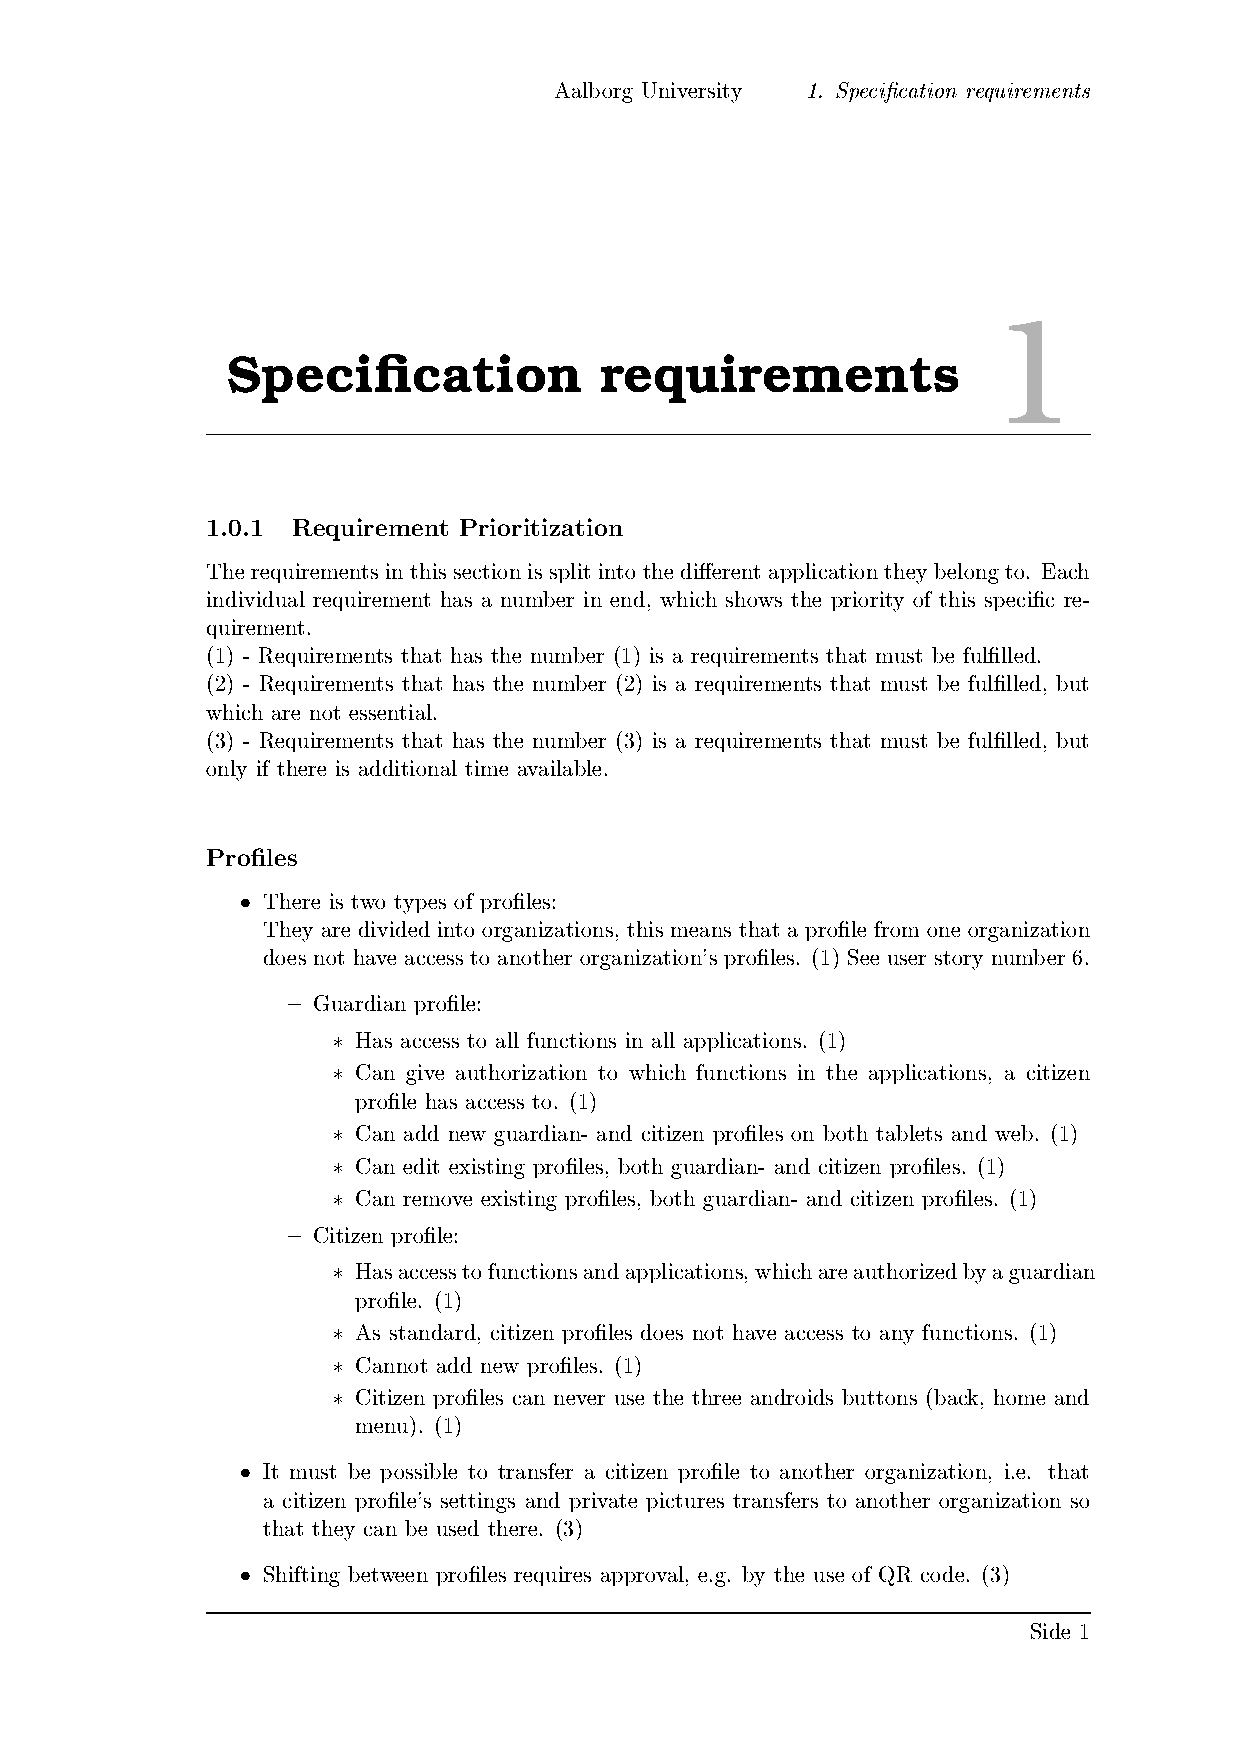
\includepdf[nup=2x2,pages={-}]{documents/Appendix/SpecificationRequirement.pdf}

\chapter{Client Meeting 01-04-2014}\label{appendix:firstmeeting}
\launcher: The point of \launcher is to foreclose the citizens from the rest of the tablets functionality.
It should be as simple as possible.
Pernille thinks it is great that one can change the profile both in the \launcher and inside each individual app.
It is nice that it is the same icon to change profiles everywhere.
There are institutions where everyone have their own tablet and others where the citizens must share.
Pernille thinks that \launcher has the nicest design demonstrated today and that the presentation of how it could work has been very good.
Settings should be individual for each citizen.
Pernille thinks it would be realistic to adjust settings inside each app.
Drazenko just wants it to work.
He believes it provides the best overview to adjust the settings inside each app as well.
However, it is very different how technically adept a citizen is.
``Generelt'' is a bad choice of words under the settings for \giraf.
Pernille wants to know why there is an ability to change colours of apps.
Drazenko thinks it is ok, but not an important feature.
It is probably a good idea to discuss with Birken and bostedet what they meant with their colour requirements.
Generally, people are leaning towards adjusting settings inside each individual app.
Drazenko thinks it is a good idea that external apps can be added to \giraf.
It must be possible to lock which applications can be chosen, so a citizen can not just play everything.
Use a different word than ``Android'', since most are used to iPads.
Another idea is to make an ``Import App'' button like when you insert pictures in a Word document.
Keep it clean and simple!
The drawer becomes irrelevant if the colours are not going to be used.
It is not clear what the purpose of the colours is.
Double check that the requirements from the groups from previous years (If you have any problems with requirements, write me a mail!)
The question is whether or not change of colours is still relevant.
An idea could be to remove the possibility of using other applications for a certain period of time, so a citizen can not switch to a different game while working with another.
Drazenko thinks that \launcher is useful and that it should be simple and grant a good overview.
It should be intuitive how the drawer is opened for change of colour.
Go out and test with the users!
Do not say anything, but observe how they are using it. 
That is really good feedback.
Take pictures so you get some great feedback.

\chapter{Client Meeting 03-04-2014}\label{appendix:secondmeeting}
Check if Android has a feature similar to Apples' ``Restricted Access''.
They like the idea regarding blocking access to other applications while the ``Timer'' is running.
They like the idea regarding profile selection in both \launcher and the individual applications.
They would prefer accessing the settings inside the individual applications.
They like the idea of a collection of settings in \launcher, but they would prefer to have it inside the applications.
They like the feature of creating setting for the guardian and being able copy settings onto the citizen profiles.
They would like both.
They like the idea of being able to bring external applications into \launcher.
They particularly like the idea of disabling and enabling applications for different citizens.
Birken thinks it is okay to see who is logged in.
To change the colours of applications is not a requirement for them.
It is fine with different colours on the applications, but changing colours is not important.

\chapter{Front End Applications}\label{sec:giraf:applications:frontend}
This appendix describes all front end applications in the \giraf suite.

\paragraph{\launcher}
provides an interface for accessing the other tablet applications in a controlled environment, that is easy to use for both guardians and citizens. 
Through \launcher, the guardians should be able to control what applications the citizens should be allowed to use. In the application interface, \launcher is referred to as \giraf.

\paragraph{Sekvens}
allows users to build sentences from pictograms, a central activity in the lives of the citizens \giraf is made to service. Many citizens with autism, especially young children, have difficulty formulating sentences in speech. A central feature of \textit{Sekvens} is also the possibility to save often used sequences of pictograms.

\paragraph{Pictooplæser}
is similar to \textit{Sekvens}, but is focused on building more ad hoc sentences, which the application is then able to read aloud using either an existing recording, or an online text-to-speech tool. 

\paragraph{Kategoriværktøjet}
allows guardians to manage the categories into which the pictograms are organised, including adding and deleting categories and subcategories.

\paragraph{Oasis App}
is an administration tool for manipulating the user information in the database. 

\paragraph{Pictosearch}
is not used as a standalone application, but provides other applications with a common interface for searching through the device's collection of pictograms.

\paragraph{Pictotegner}
allows the user to create their own pictograms with basic graphics tools, such as a free-hand pen tool, a rectangle tool, a circle tool etc. 

\paragraph{Livshistorier}
is also similar to \textit{Sekvens}, but is created specifically for saving pictogram sequences that contain instructions for the citizen's everyday life, e.g. instructions on how to use the bathroom.

\paragraph{Ugeplan}
allows the users to build weekly activity schedules using pictograms. Autistic citizens thrive best in highly strutured environments with regularly scheduled days.

\paragraph{Tidstager}
provides the ability to time an activity, allowing a guardian to let a citizen use an application, e.g. a game, for a set amount of time. When the time runs out, the device locks, forcing the citizen to move on to the next scheduled activity.

\paragraph{Stemmespillet}
is a game, where the citizen controls a car by varying the volume of his or her voice. 

\paragraph{Kategorispillet}
is a game, where the citizen unloads pictograms from a train. The pictograms must be unloaded at different stations, where each station accepts a certain category of pictograms.

\paragraph{Web Ugeplan}
is a web-version of \textit{Ugeplan}, specifically design for large touchscreens. A few costumers had access to TV-size touchscreen, which they specifically wished to use for their week schedules.

\paragraph{Webadmin}
is a web-based administration tool for manipulating the user information in the database.

\chapter{Further code examples}\label{appendix:codeexamples}
This appendix contains code fragments, that are too big to be included as part of the report and that can be omitted..

\section {Debug mode for development}\label{appendix:debugmode}
This section describes the implementation of a debug mode, making developers able to skip certain steps in \launcher, such as the animation screen and the authentication screen.\\

When opening \launcher one is presented \mainactivity, which shows a loading animation, while loading data from the remote database\footnote{Please note, that because the remote database synchronisation was enabled so late in the fourth sprint, debug mode has not been tested.}.
\launcher also requires the users to authenticate themselves, before being given access to the \homeactivity.
While these activities hold meaning in the context of the intended users, a significant amount of debugging time is wasted, as the application is often reinstalled and restarted during development. 

To overcome this problem, we decided to implement a debug mode to simplify and quicken the process of working with \launcher.
The debug mode is controlled from the source code \lstinline|MainActivity| by setting the local fields below (thus, it is not possible to control debug mode at runtime):

\begin{itemize}
\item Enable (true) or disable (false) debug mode entirely, overriding other settings:\\
\lstinline|private final boolean DEBUG_MODE = true;|
\item Skip \lstinline|AuthenticationActivity| activity:\\
\lstinline|private final boolean showAuthentication = false;|
\item Skip the animation on \lstinline|MainActivity| activity:\\
\lstinline|private final boolean showMainAnimation = false;|
\item Login either as a guardian or child when skipping authentication:\\
\lstinline|private final boolean loginAsChild = false;|
\end{itemize}

When the above fields are set, debug mode is enabled globally in \launcher from the \lstinline|onCreate()| method in \lstinline|MainActivity| through the call showed in \cref{lst:debugmode:enable}.

\begin{lstlisting}[caption={Enable debug mode from \lstinline|MainActivity|.},label={lst:debugmode:enable}]  
if(DEBUG_MODE)
  LauncherUtility.enableDebugging(DEBUG_MODE, loginAsChild, this);
\end{lstlisting}

The \lstinline|enableDebugging()| method is seen in \cref{lst:debugmode:enablemethod}.
It needs a reference of the calling activity to show debug information in the active activity.

\begin{lstlisting}[caption={Enable debug mode by calling \lstinline|enableDebugging()|.},label={lst:debugmode:enablemethod}]  
public static void enableDebugging(boolean debugging, boolean loginAsChild, Activity activity) {
  DEBUG_MODE = debugging;
  DEBUG_MODE_AS_CHILD = loginAsChild;

  ShowDebugInformation(activity);
}
\end{lstlisting}

The code in \cref{lst:debugmode:show} is used to set the necessary views, as to inform the developer that debug mode is enabled.

\begin{lstlisting}[caption={Show a debug information on activity if debug is enabled.},label={lst:debugmode:show}]  
public static void ShowDebugInformation(Activity a) {
  if (DEBUG_MODE) {
    LinearLayout debug = (LinearLayout) a.findViewById(R.id.debug_mode);
    TextView textView = (TextView) a.findViewById(R.id.debug_mode_text);
    textView.setText(a.getText(R.string.giraf_debug_mode) + " " + (DEBUG_MODE_AS_CHILD ? a.getText(R.string.giraf_debug_as_child) : a.getText(R.string.giraf_debug_as_guardian)));
    debug.setVisibility(View.VISIBLE);
    try {
      Thread.sleep(200);
    } catch (InterruptedException e) {
      e.printStackTrace();
    }
  }
}
\end{lstlisting}


\section{Launching Google Play}

The code in \cref{lst:launchergoogleplay} describes the \lstinline|OnClickListener| for the \textbf{''Butik''} button in the ''Apps'' pane of settings.
It attempts to open the Play Store app - If it is not installed on the device, it opens Play Store in the browser instead.
\begin{lstlisting}[caption={The OnClickListener for the googlePlayButton, launching the Play Store correctly}, label={lst:launchergoogleplay}]
googlePlayButton.setOnClickListener(new View.OnClickListener() {
	public void onClick(View v) {
		// Try to start the Google Play app
		try {
			Intent intent = new Intent();
			intent.setData(Uri.parse(MARKET_SEARCH_APP_URI + PUBLISHER_NAME));
			intent.setFlags(Intent.FLAG_ACTIVITY_NEW_TASK | Intent.FLAG_ACTIVITY_CLEAR_TOP);
			startActivity(intent);
			// If Google Play is not found, parse the url for Google Play website
		} 
		catch (android.content.ActivityNotFoundException e) {
			startActivity(new Intent(Intent.ACTION_VIEW, Uri.parse(MARKET_SEARCH_WEB_URI + PUBLISHER_NAME)));
		}
	}
}
\end{lstlisting}

\section{Derived class of LoadApplicationTask}

\cref{lst:derivedlat} shows the \lstinline|LoadGirafApplicationTask| - a derived class of \lstinline|LoadApplicationTask|.
The methods of the class calls \lstinline|super.fooBar()| to let the super class carry out most of the work, along with initiating the \lstinline|AppUpdater| in that class and specifying which applications to load.

  \begin{lstlisting}[caption={The LoadGirafApplicationTask, derived from LoadApplicationTask. This is the derived class used by GirafFragment to load applications into view. Please note that all comments and the constructor have been removed to make the listing smaller}, label={lst:derivedlat}]
class LoadGirafApplicationTask extends LoadApplicationTask {
	
	@Override
	protected void onPreExecute() {
		if(appsUpdater != null)
		appsUpdater.cancel();
		
		super.onPreExecute();
	}
	
	@Override
	protected HashMap<String, AppInfo> doInBackground(Application... applications) {
		apps = ApplicationControlUtility.getGirafAppsOnDeviceButLauncherAsApplicationList(context);
		applications = apps.toArray(applications);
		appInfos = super.doInBackground(applications);
		
		return appInfos;
	}
	
	@Override
	protected void onPostExecute(HashMap<String, AppInfo> appInfos) {
		super.onPostExecute(appInfos);
		loadedApps = appInfos;
		startObservingApps();
		haveAppsBeenAdded = true;
	}
}
\end{lstlisting}

\section{Marking GIRAF and Android applications}\label{appendix:markingapps}

\cref{lst:addinggirafapplications} contains the code for marking \giraf applications in the ''Apps'' pane of settings, while \cref{lst:addingandroidapplications} contains the code for marking Android applications in the same pane.

\begin{lstlisting}[caption={The methods used for adding or removing a Giraf application to a user}, label={lst:addinggirafapplications}]
ProfileApplicationController pac = new ProfileApplicationController(context);
ProfileApplication pa = new ProfileApplication(currentUser.getId(), app.getApp().getId());
if(pa == null)
	pac.insertProfileApplication(pa);
else
	pac.removeProfileApplicationByProfileAndApplication(app.getApp(), currentUser);
\end{lstlisting}

\begin{lstlisting}[caption={The methods used for adding or removing an Android application to a user. Please note that the documentation has been removed.}, label={lst:addingandroidapplications}]
String activityName = app.getActivity();

if (selectedApps.contains(activityName))
    selectedApps.remove(activityName);
else
    selectedApps.add(activityName);
\end{lstlisting}

\chapter{Remaining Backlog}\label{appendix:futureworks}
This appendix contains information about the things still remaining to be done in the \launcher project.
As such, it acts as a backlog for the next year bachelor students working on the project.

\section{Proper iconsize}
When scaling the application icons some of them gets pixellated, this indicates that there is still work to be done, when choosing the icons to show. This might be caused by low resolution icons supplied by the developers of the other applications.

\section{Ugeskema Calendarwidget}
The group working on the \textit{GIRAF components} has a widget, showing the current date, in their backlog and it would be an idea to use this widget to open the application \textit{Ugeplan} through this widget. The application should then show the schema for the citizen chosen from the profile selector.

\section{Logging in with citizen and administrator profiles}
Currently, it is possible to login with all types of profiles, but there is no handling of types other than guardian profiles in most of the application.
It might be needed for citizen and administrator login as well.
Citizen profiles should not be able to access certain activities, such as settings in \launcher.
On the contrary, the administrator profiles would need additional access to system administration applications.

\section{Automatically download \giraf applications}
It could be nice to have the \launcher start downloading all \giraf applications as soon as it is started.
This is most likely not possible in Android but it is possible to start Google Play with a search string, meaning that it could be possible to start Google Play with the common part of the Java package name used for the \giraf applications.

\section{Add sound to Launcher}
Currently, none of the actions a user carries out when using \launcher provides audio feedback.
Adding minor sounds for button presses, application launching, setting changes and the like, could be a nice touch to add to \launcher. 

\section{Profile Selection Dialog}
It should be clearly indicated what role, the individual user is assigned, in the list when opening the profile selection dialog.
Currently there are no indication of the role of a user.

\section{Copying settings from one user to another}
For many citizens, the settings may be quite similar.
For this reason, it would be preferable to be able to copy settings from one user to another.

\section{Authentication Activity}
There are still work to do in the authentication activity.

\begin{itemize}
	\item Make it clear that the QR code was successfully scanned.

	An idea is that the camera feed is hidden when the QR code is accepted and who buttons are show, one to scan again and one to login.
	\item Rotation of the instruction animation.

	Currently it is shown as the tablet should be held in portrait mode. For usability matters this should be rotated. %Good luck and have fun with this...!
\end{itemize}

\section{Download pictograms while tablet is being used}
When \launcher is started after a reboot of the device the synchronisation i of data with the remote database is done before being able to login.
If \launcher has never been installed on the device before, this means that it can take up to 30 minutes, before it is ready to login.
It would be an idea to only load the necessary information such as profiles, and then continue downloading the pictograms in the background while the tablet is being used.

\section{GridView used for loading applications}
The container in which applications are being loaded is implemented inconveniently. It should be implemented with a grid view, using a custom adapter. This is better for memory management, and would simplify the algorithm used for showing applications. \frederik{ref til stefans afsnit om adapter i settings}

\label{totalpage}

% Bibliography
\label{biblo}
\bibliography{sources}

%Count the last page	
\label{lastpage}
\end{document}